
\documentclass[12pt]{article}

%	页面设置
\usepackage{geometry}
\geometry{left=2.5cm, right=2.5cm, top=2.5cm, bottom=2.5cm}
\usepackage{graphicx}
\usepackage{ctex}
\usepackage{fontspec}
\usepackage{setspace}
\usepackage{array,longtable,subcaption,multirow,float,calc,tcolorbox}
\usepackage{siunitx}
\usepackage[version=4]{mhchem}
\usepackage{inconsolata}
\usepackage[strict]{changepage}
\usepackage{listings}
\usepackage{xcolor} % for setting colors

% Define your colors here
\definecolor{codegray}{gray}{0.9}

% Set up the listings package to format the code
\lstnewenvironment{code}{
    \lstset{
        backgroundcolor=\color{codegray}, % set the background color
        basicstyle=\ttfamily, % set the font style to teletype family
        breaklines=true, % allows line breaking
        numbers=left, % line numbers on the left
        numberstyle=\tiny\color{gray}, % style for the line numbers
        stepnumber=1, % numbering steps
        numbersep=5pt, % how far the line numbers are from the code
        frame=none, % no frame around the code
        framesep=0pt, % space before and after the code (if no frame, not needed)
        rulecolor=\color{black}, % frame color (if no frame, not needed)
        framerule=0pt, % frame thickness (if no frame, not needed)
        fillcolor=\color{codegray}, % background color (if not using the general backgroundcolor)
        tabsize=4, % tab size
        showstringspaces=false, % don't mark spaces in strings
        aboveskip=1pt, % reduces the default spacing above the code block
        belowskip=2pt, % reduces the default spacing below the code block
        % any other code settings can be added here
    }
}{}



%\usepackage{etoolbox}
%\robustify\ref
%\pretocmd{\ref}{\textbf}{}{}

%	字体设置
\setmainfont{Times New Roman}
\setCJKmainfont{SimSun.ttf}
\setCJKsansfont{SimHei.ttf}

%	表格设置
\usepackage{makecell}
\newcommand{\addcell}[2][4]{\makecell{\zihao{#1}\textsf{#2}}}
\usepackage{titlesec}
\usepackage{booktabs}
\usepackage{tabularx}

%	设置图注、表注
\usepackage{caption}
\usepackage{bicaption}
\captionsetup{labelsep=quad, font={small, bf}, skip=2pt}
\DeclareCaptionOption{english}[]{
    \renewcommand\figurename{Fig.}
    \renewcommand\tablename{Table}
}
\captionsetup[bi-second]{english}

%	设置页眉
\usepackage{fancyhdr}
\pagestyle{fancy}
\fancypagestyle{preContent}{
    \fancyhead[L]{\zihao{-5} 物理化学实验}
    \fancyhead[C]{\zihao{-5} 物理化学实验期末小结}
    \fancyhead[R]{\zihao{-5} 2100011873\ 王子宸}
}
\pagestyle{preContent}

%	设置首页页眉及取消首页页脚 若不需要首页页眉 请注释掉下列内容
%\fancypagestyle{plain}{
	%\fancyhead[L]{\zihao{-5} 物理化学实验}
	%\fancyhead[C]{\zihao{-5} 实验xx\ \ xxxxx}
	%\fancyhead[R]{\zihao{-5} xxxxxxxxxx\ xxx}
	%\cfoot{}
%}

%	设置标题格式
\titleformat*{\section}{\zihao{4}\sffamily}
\titleformat*{\subsection}{\zihao{-4}\sffamily}
\titleformat*{\subsubsection}{\zihao{-4}\sffamily}
\titlespacing*{\section}{0pt}{10pt}{10pt}
\titlespacing*{\subsection}{0pt}{10pt}{5pt}
\titlespacing*{\subsubsection}{0pt}{10pt}{5pt}

%	设置引用格式(ACS格式规范)
%	注意:请安装JabRef
%	JabRef使用参考:https://blog.csdn.net/weixin_44191286/article/details/85698921
\usepackage[super,round,comma,compress]{natbib}

%	数学公式增强
\usepackage{amsmath}
\usepackage{amssymb}

\newcolumntype{M}[1]{>{\centering\arraybackslash}m{#1}}
%	设置封面
\begin{document}
    % 标题页

\begin{titlepage}
% 页眉
\thispagestyle{plain}
% 校徽图片
\begin{figure}[h]
    \centering
    \includegraphics{pku.png}
\end{figure}
\vspace{24pt}
% 标题
\centerline{\zihao{-0} \textsf{物理化学实验报告}}
\vspace{40pt} % 空行
\begin{center}
    \begin{tabular}{cc}
        % 题目
        
        \addcell[2]{题目:\ } & \addcell[2]{紫外可见吸收光谱仪的搭建 与} \\
        \cline{2-2}\\
        & \addcell[2]{量子一维势阱方程的检验}\\
        \cline{2-2}
        
    \end{tabular}
\end{center}
\vspace{20pt} % 空行
\begin{center}
    \doublespacing
    \begin{tabular}{cp{5cm}}
        % 姓名
        \addcell{姓\phantom{空格}名:\ } & \addcell{王子宸} \\
        \cline{2-2}
        % 学号
        \addcell{学\phantom{空格}号:\ } & \addcell{2100011873}\\
        \cline{2-2}
        % 组别
        \addcell{组\phantom{空格}别:\ } & \addcell{周四19组8号} \\
        \cline{2-2}
        % 实验日期
        \multirow{2}{*}{\addcell{实验日期:\ }} & \addcell{\zhdate{2023/10/26}}\\
        \cline{2-2}
        & \addcell{\zhdate{2023/11/2}}\\
        \cline{2-2}
        % 室温
        \addcell{室\phantom{空格}温:\ } & \addcell{20.6\si{^\circ C}\ \ 21.7\si{^{\circ}C}}\\
        \cline{2-2}
        % 大气压强
        \addcell{大气压强:\ } & \addcell{100.95\si{kPa}\quad99.90\si{kPa}}\\
        \cline{2-2}
    \end{tabular}
    \begin{tabular*}{\textwidth}{c}
    \\
    \\
        \hline % 分割线
    \end{tabular*}
\end{center}
% 摘要
\textsf{摘\ \ 要}\ \ 本实验利用实验室提供的部件搭建了紫外可见吸收光谱仪,利用氘灯对光谱仪进行了调试和标定;用光谱仪测定了同一物质不同浓度溶液的吸收光谱,拟合工作曲线,验证了 Lambert-Beer 定律,并对比了使用氘灯光源和卤钨灯光源的差异;测量了多个共轭分子的吸收光谱,计算了各分子的摩尔吸光系数 $\varepsilon $;分别用一维势阱模型和 Gaussian 程序对各分子进行了模拟计算,比较了计算结果与实验结果的差别。
\\
\\
% 关键字
\textsf{关键词}\ \ 物理化学实验;紫外-可见吸收光谱仪;一维势阱模型;花菁染料;TDDFT
\end{titlepage}

\section{引言}

\subsection{实验目的与原理}

\begin{figure}[H]
    \centering
    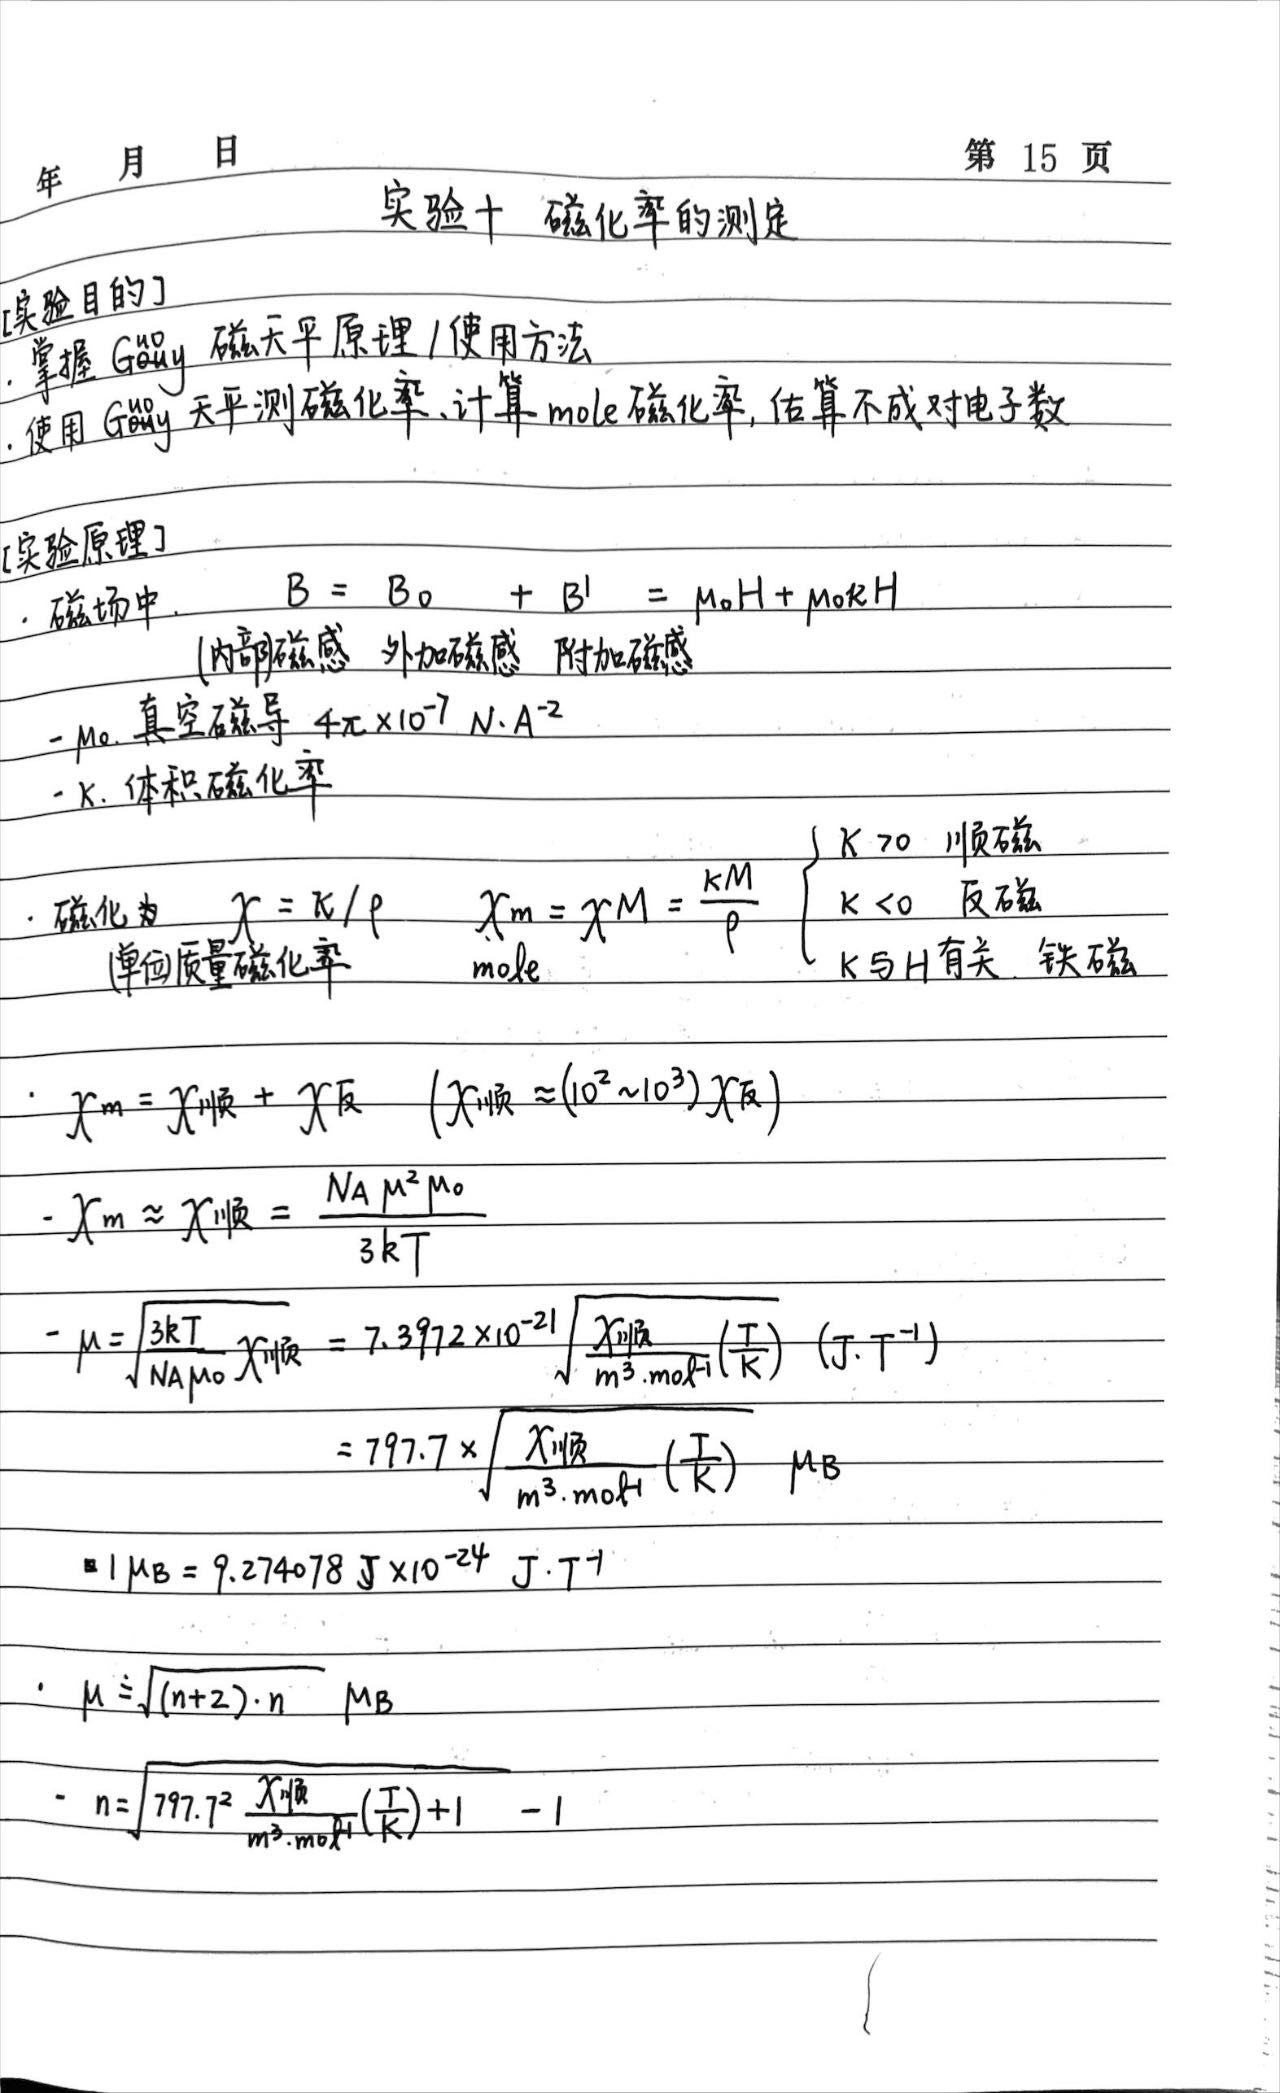
\includegraphics[width=.8\textwidth]{figures/0-1.jpg}
    \bicaption{预习报告:实验的目的与原理(1)}{Preview Report: Purpose and Principle of the Experiment 1}
\end{figure}

\begin{figure}[H]
    \centering
    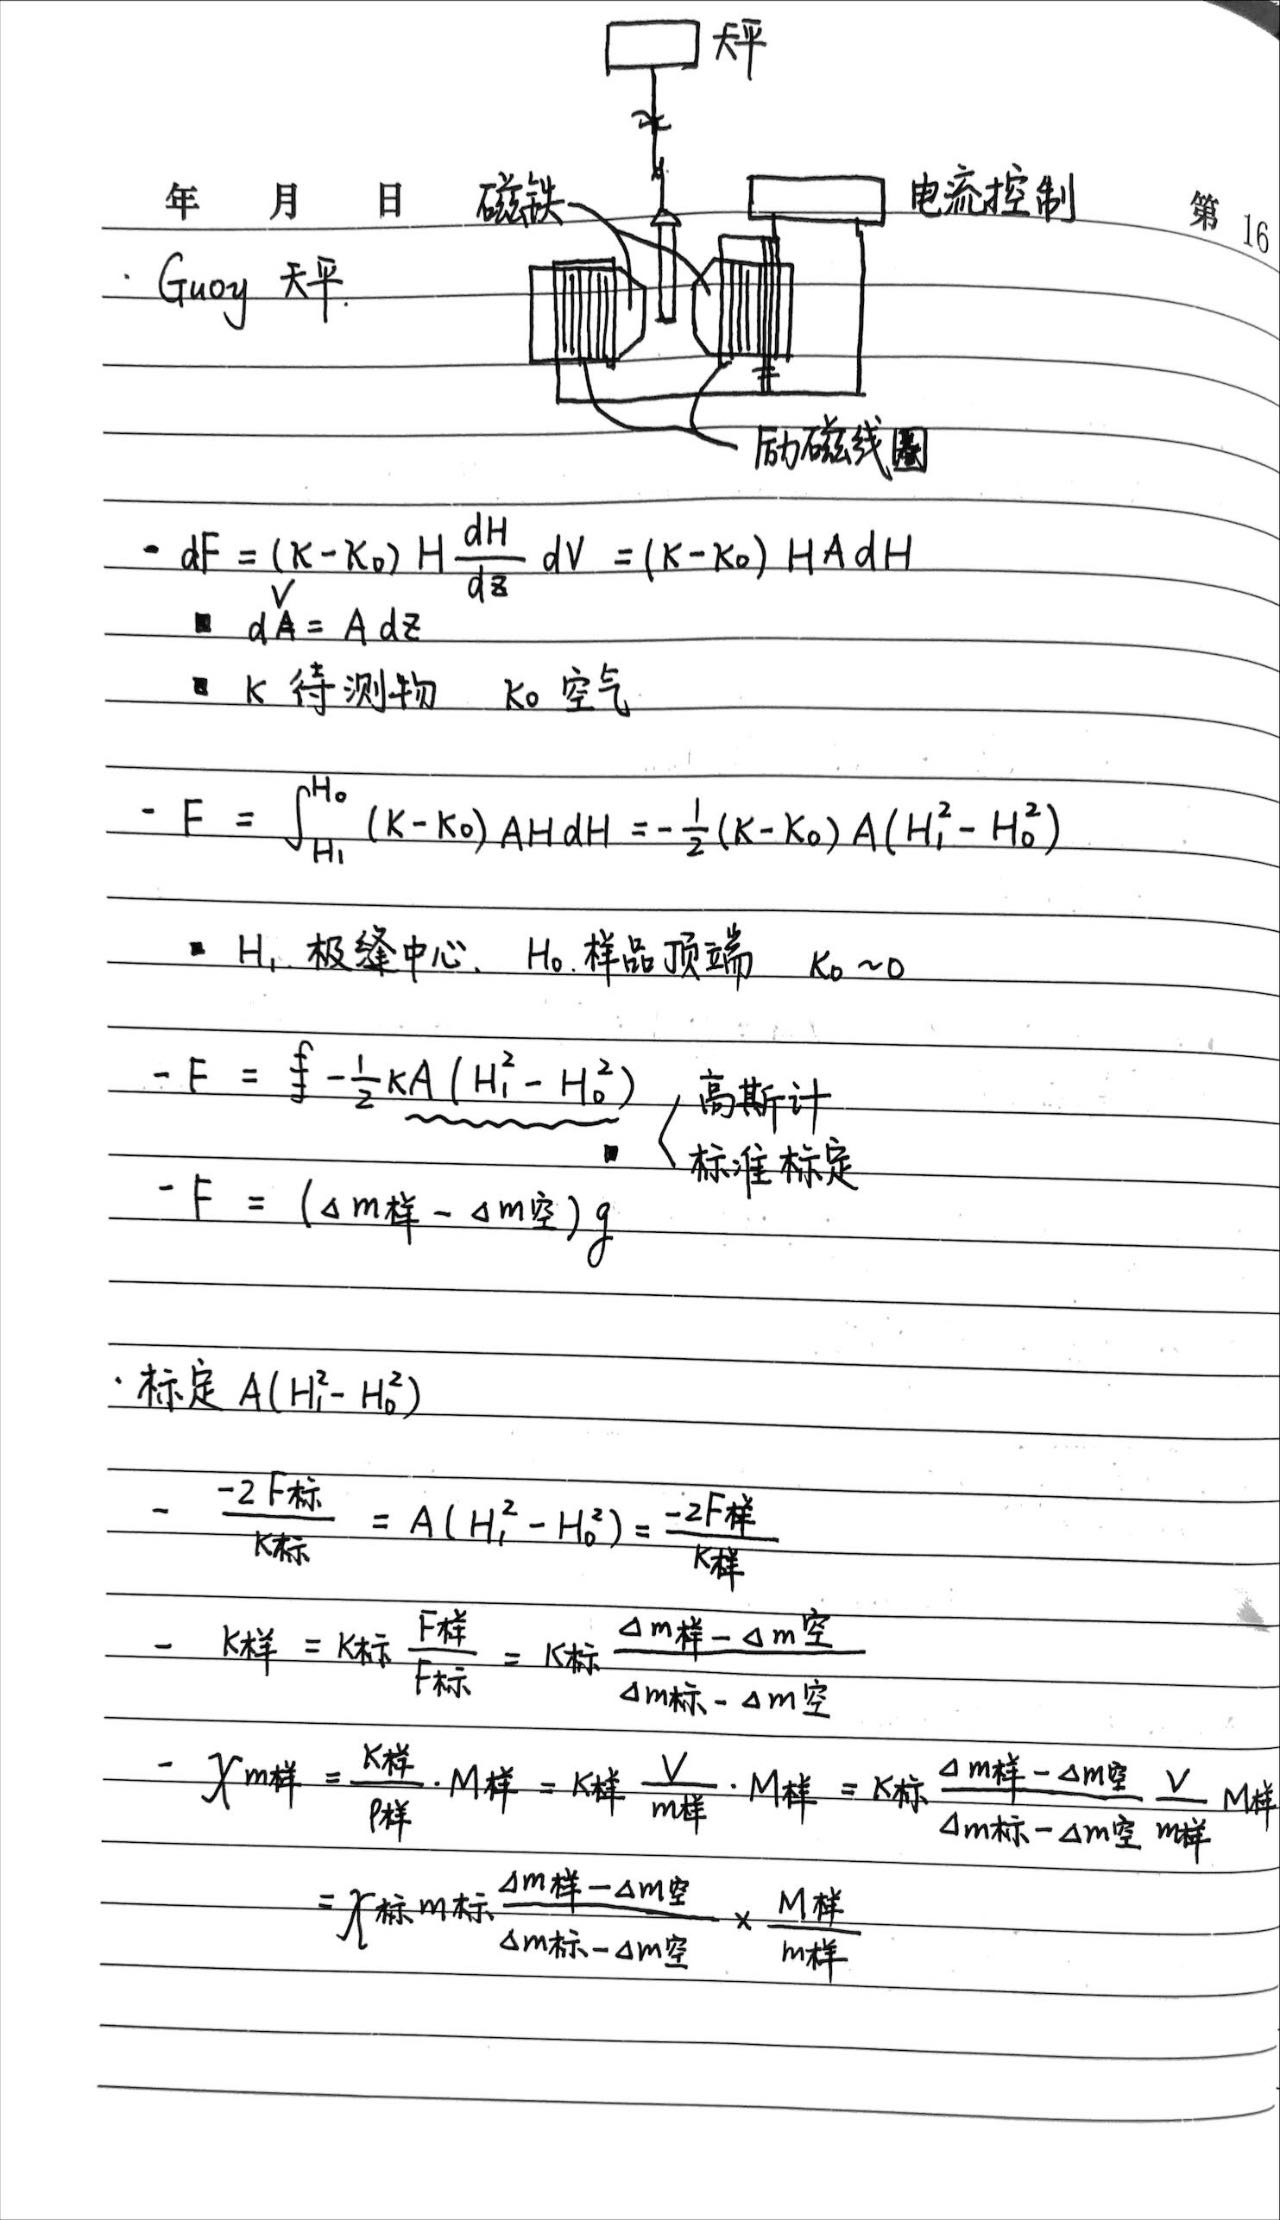
\includegraphics[width=.8\textwidth]{figures/0-2.jpg}
    \bicaption{预习报告:实验的目的与原理(2)}{Preview Report: Purpose and Principle of the Experiment 2}
\end{figure}




\end{document}